\documentclass [a4paper,10pt] {article}
\usepackage[latin1]{inputenc}
\usepackage[ngerman]{babel}
\usepackage[T1]{fontenc}
\usepackage{amsmath, amsthm, amssymb}
\usepackage{latexsym}
\usepackage{graphicx}
\usepackage{a4wide}
\setlength{\parindent}{0mm}
\setlength{\parskip}{3mm}
\usepackage{fancyhdr}
\renewcommand{\labelenumi}{(\alph{enumi})}
\pagestyle{fancy}
\headheight 16pt
\renewcommand{\headrulewidth}{0.4pt}
\renewcommand{\footrulewidth}{0.4pt}
\renewcommand{\familydefault}{\sfdefault}
\lhead{Lego Mindstorms Praktikum}
\chead{Team A}
\rhead{SS 2010}
\begin{document}
%\pagestyle{empty}%
%\tableofcontents %
%\newpage%

%content ab hier
%\begin{description}
%	\item[] \emph{} $\rightarrow$ 
%	\includegraphics[width=10cm]{}
% \end{description} 

\section{Vor�berlegungen}
\subsection{Aufgabenstellung}
Es sind Robotor zu konstruieren, die ein Sokoban-Spiel zun�chst einlesen und dann l�sen. Zu den Regeln eines normalen Sokoban--Spiels wird hierbei zus�tzlich zu dem Schieber ein Zieher eingesetzt. Au�erdem wird ein Kartierer ben�tigt und ein Bauteil, dass die L�sung des Spiels berechnet. \\
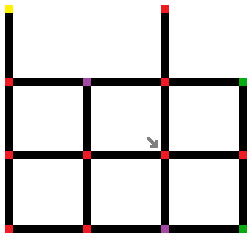
\includegraphics[width=10cm]{soko.png} \\
Das Feld besteht aus schwarzen Linien. Die Kreuzungen sind durch verschiedene Faben gekennzeichnet. Gr�n steht f�r die Ziele der Kisten, Violett f�r die Startr�ume, Gelb f�r den Startraum des Schiebers und ein Pfeil markiert den Startraum des Ziehers und des Kartierers. Rot wird f�r normale Kreuzungen verwendet. 
\subsection{Zeitplan}
	\textbf{Beginn:} 10. September 2010 \\
	\textbf{Abgabe:} 27. September 2010
	
	\textbf{Konstruktion der Roboter:} ca. 1 Tag \\
	\textbf{Testen von Sensoren und anderen Komponenten:} ca. 2 Tage \\
	\textbf{Implementierung der zusammenfassenden Navigation:} ca. 2 Tage \\
	\textbf{Implementierung des Kartierers:} ca. 3-4 Tage \\
	\textbf{Implementierung des Planers:} ca. 4-5 Tage \\
	\textbf{Implementierung des Ziehers:} ca. 3 Tage \\
	\textbf{Implementierung des Schiebers:} ca. 3 Tage \\
	\textbf{Testen und Optimierung:} ca. 3-4 Tage	
\subsection{Aufgabenverteilung}
	\textbf{Teammitglieder:} \\
Till Rohrmann, Wiebke K�pp, Christoph Bruns, Michael Bigontina, Andreas Bigontina, Anastasia Panteloglou, Maximilian Burger, Sebastian Hagen

	\textbf{Organisation:} \\ 
Till Rohrmann, Wiebke K�pp \\
	\textbf{Kartierer:} \\ 
Maximilian Burger, Sebastian Hagen \\
	\textbf{Planer:} \\
Till Rohrmann, Wiebke K�pp \\ 
	\textbf{Zieher:} \\
Christoph Bruns, Michael Bigontina \\	
	\textbf{Schieber} \\ 
Andreas Bigontina, Anastasia Panteloglou 
\subsection{L�sungsansatz}
	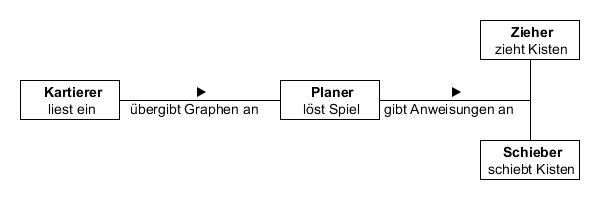
\includegraphics[width=13cm]{sol.jpg} \\
	Kartierer:
	\\
	Planer: 
	\\
	Schieber:
	\\
	Zieher:

%\section{Verlauf}

%\subsection{Freitag, 10.09.2010} 
%	\begin{itemize}
%	\item Geplante Schritte:
%		\begin{itemize}
%			\item Github und Laptops einrichten um mobiler zu sein
%			\item Farb -- und Lichtsensoren testen (Till Rohrmann)
%			\item Kartierer bauen (Sebastian Hagen, Maximilian Burger, Wiebke K�pp)
%			\item Zieher bauen (Christoph Bruns, Michael Bigontina)
%			\item Schieber bauen (Andreas Bigontina, Anastasia Pantaleglou)
%			\item Navigator programmieren (Till Rohrmann, Sebastian Hagen, Maximilian Burger)
%			\item Robotoreigenschaften testen (Wiebke K�pp)   
%			\item (zu Beginn: vervollst�ndigen verbleibender Einf�hrungsaufgaben)
%		\end{itemize}
%	\item Tats�chlicher Fortschritt:
%		 \begin{itemize}
%			\item --
%		\end{itemize}
%\end{itemize}

% \subsection{Montag, 13.09.2010}
%	\begin{itemize}
%	\item Geplante Schritte:
%		\begin{itemize}
%			\item 
%			\item 
%			\item  
%		\end{itemize}
%	\item Tats�chlicher Fortschritt:
%		 \begin{itemize}
%			\item 
%		\end{itemize}
%\end{itemize}



\end{document}